%%%%%%%% ICML 2021 EXAMPLE LATEX SUBMISSION FILE %%%%%%%%%%%%%%%%%

\documentclass{article}
\usepackage{float}
\usepackage{microtype}
\bibliographystyle{icml2021}
\usepackage{graphicx}
\usepackage{subfigure}
\usepackage{booktabs}
\usepackage{float}
\usepackage{gensymb}
\usepackage{amsmath}
\usepackage{amssymb}
\usepackage{tikz}

\usepackage{url}
\def\UrlBreaks{\do\/\do-}
\usepackage{breakurl}
\usepackage[breaklinks]{hyperref}
\usepackage{hyperref}

\newcommand{\theHalgorithm}{\arabic{algorithm}}
\newcommand{\TODO}[1]{\textcolor{blue}{#1}}

\usepackage[accepted]{icml2021}

\icmltitlerunning{Hyperparameter Tuning using Evolutionary Algorithms}

\begin{document}

\twocolumn[
\icmltitle{Hyperparameter Tuning using Evolutionary Algorithms}
\icmlsetsymbol{equal}{*}
\begin{icmlauthorlist}
    \icmlauthor{T. Blom (sXXXXXXXX)}{LIACS}
    \icmlauthor{J. Hamelink (s2233827)}{LIACS}
    \icmlauthor{L. Peeters (sXXXXXXX)}{LIACS}
    \icmlauthor{S. Sharma (sXXXXXXX)}{LIACS}
\end{icmlauthorlist}
\icmlaffiliation{LIACS}{LIACS, Leiden University, Leiden, Netherlands}
\icmlcorrespondingauthor{Mike Preuss}{LIACS}
\icmlkeywords{Hyperparameter Tuning, Evolutionary Algorithms, Reinforcement Learning}

\vskip 0.3in
]

\printAffiliationsAndNotice{}

% -------------------------------------------------------------------
% -------------------------------------------------------------------
\section{Introduction}
\label{sec:intro}

\TODO{RL is tough bc HPO, so we do EA to automate HPO. We test using gym envs. Our agent is A2C.}

% -------------------------------------------------------------------
% -------------------------------------------------------------------
\section{Methodology}
\label{sec:meth}

\TODO{small intro for this section.}

% -------------------------------------------------------------------
\subsection{Actor-Critic}
\label{ssec:ac}

\TODO{
    We do AC and A2C.
    Pseudo-code and equations.
    Explain methods: 2-headed neural network, entropy regularization, advantage estimation.
    Mention that these params will be tuned using EA.
}

We don't use this paper, but it's just to show that the citations work \cite{han2020actorcritic}.

% EXAMPLE ALGORITHM
\begin{algorithm}[htbp]
    \caption{Actor-Critic}
    \label{alg:trunk}
    \begin{algorithmic}[1]
        \STATE {\bfseries Input:} environment, $\pi_\theta$, $V_\phi$
        \STATE \texttt{$\pi_\theta$} $\gets$ random values
        \STATE \texttt{$V_\phi$} $\gets$ random values
        
        \WHILE {not converged}
            \STATE Under policy $\pi_\theta$,
            \STATE sample episode $s_0, a_0, r_1, \dots, s_{T-1}, a_{T-1}, r_T$
            \STATE \texttt{G} $\gets$ discounted returns using equation \ref{eq:disc-ret}
            \IF {using advantage estimation}
                \STATE \texttt{G} $\gets$ \texttt{G} - \texttt{V}
            \ELSE
                \STATE \texttt{G} $\gets$ \texttt{G}
            \ENDIF
            \STATE Update $\pi_\theta$ and $V_\phi$ using \texttt{G}
        \ENDWHILE
    \end{algorithmic}
\end{algorithm}

% EXAMPLE EQUATION
\begin{equation}
    \label{eq:disc-ret}
    G_t = \sum_{k=0}^{\infty} \gamma^k r_{t+k+1}
\end{equation}

% -------------------------------------------------------------------
\subsection{Evolutionary Algorithm}

\TODO{
    EA is a population-based search algorithm.
    Pseudo-code and equations.
    Explain methods: deterministic selection, elitism, 1-p crossover, uniform mutation.
    Do not mention the settings chosen for parameters such as $\mu, \lambda$ and mutation rate yet.
}

% EXAMPLE TABLE
\begin{table}[htbp]
    \centering
    \begin{tabular}
        {|c|c|}
        \toprule
        \textbf{Parameter} & \textbf{Value} \\
        \midrule
        population size & 6 \\
        $\mu$           & 3 \\
        $\lambda$       & 3 \\
        mutation rate   & 0.1 \\
        \bottomrule
    \end{tabular}
    \caption{Hyperparameters}
    \label{tab:hyper}
\end{table}

% -------------------------------------------------------------------
% -------------------------------------------------------------------
\section{Experiments}
\label{sec:exp}

\TODO{
    List environments: CartPole, Acrobot, LunarLander.
    Explain why these environments were chosen (discrete action space, no input that needs conv layers).
    List bitstring makeup: what values for what params.
    Don't mention results yet.
}

% -------------------------------------------------------------------
% -------------------------------------------------------------------
\section{Results}
\label{sec:res}

\TODO{
    For each of the subsections, small introduction of what is to be expected.
    Then graphs and tables.
    Then (not super in-depth) analysis of the results.
}

% -------------------------------------------------------------------
\subsection{CartPole}
\label{ssec:cp}

\TODO{Lorem ipsum.}

% EXAMPLE FIGURE
\begin{figure}[htbp]
    \centering
    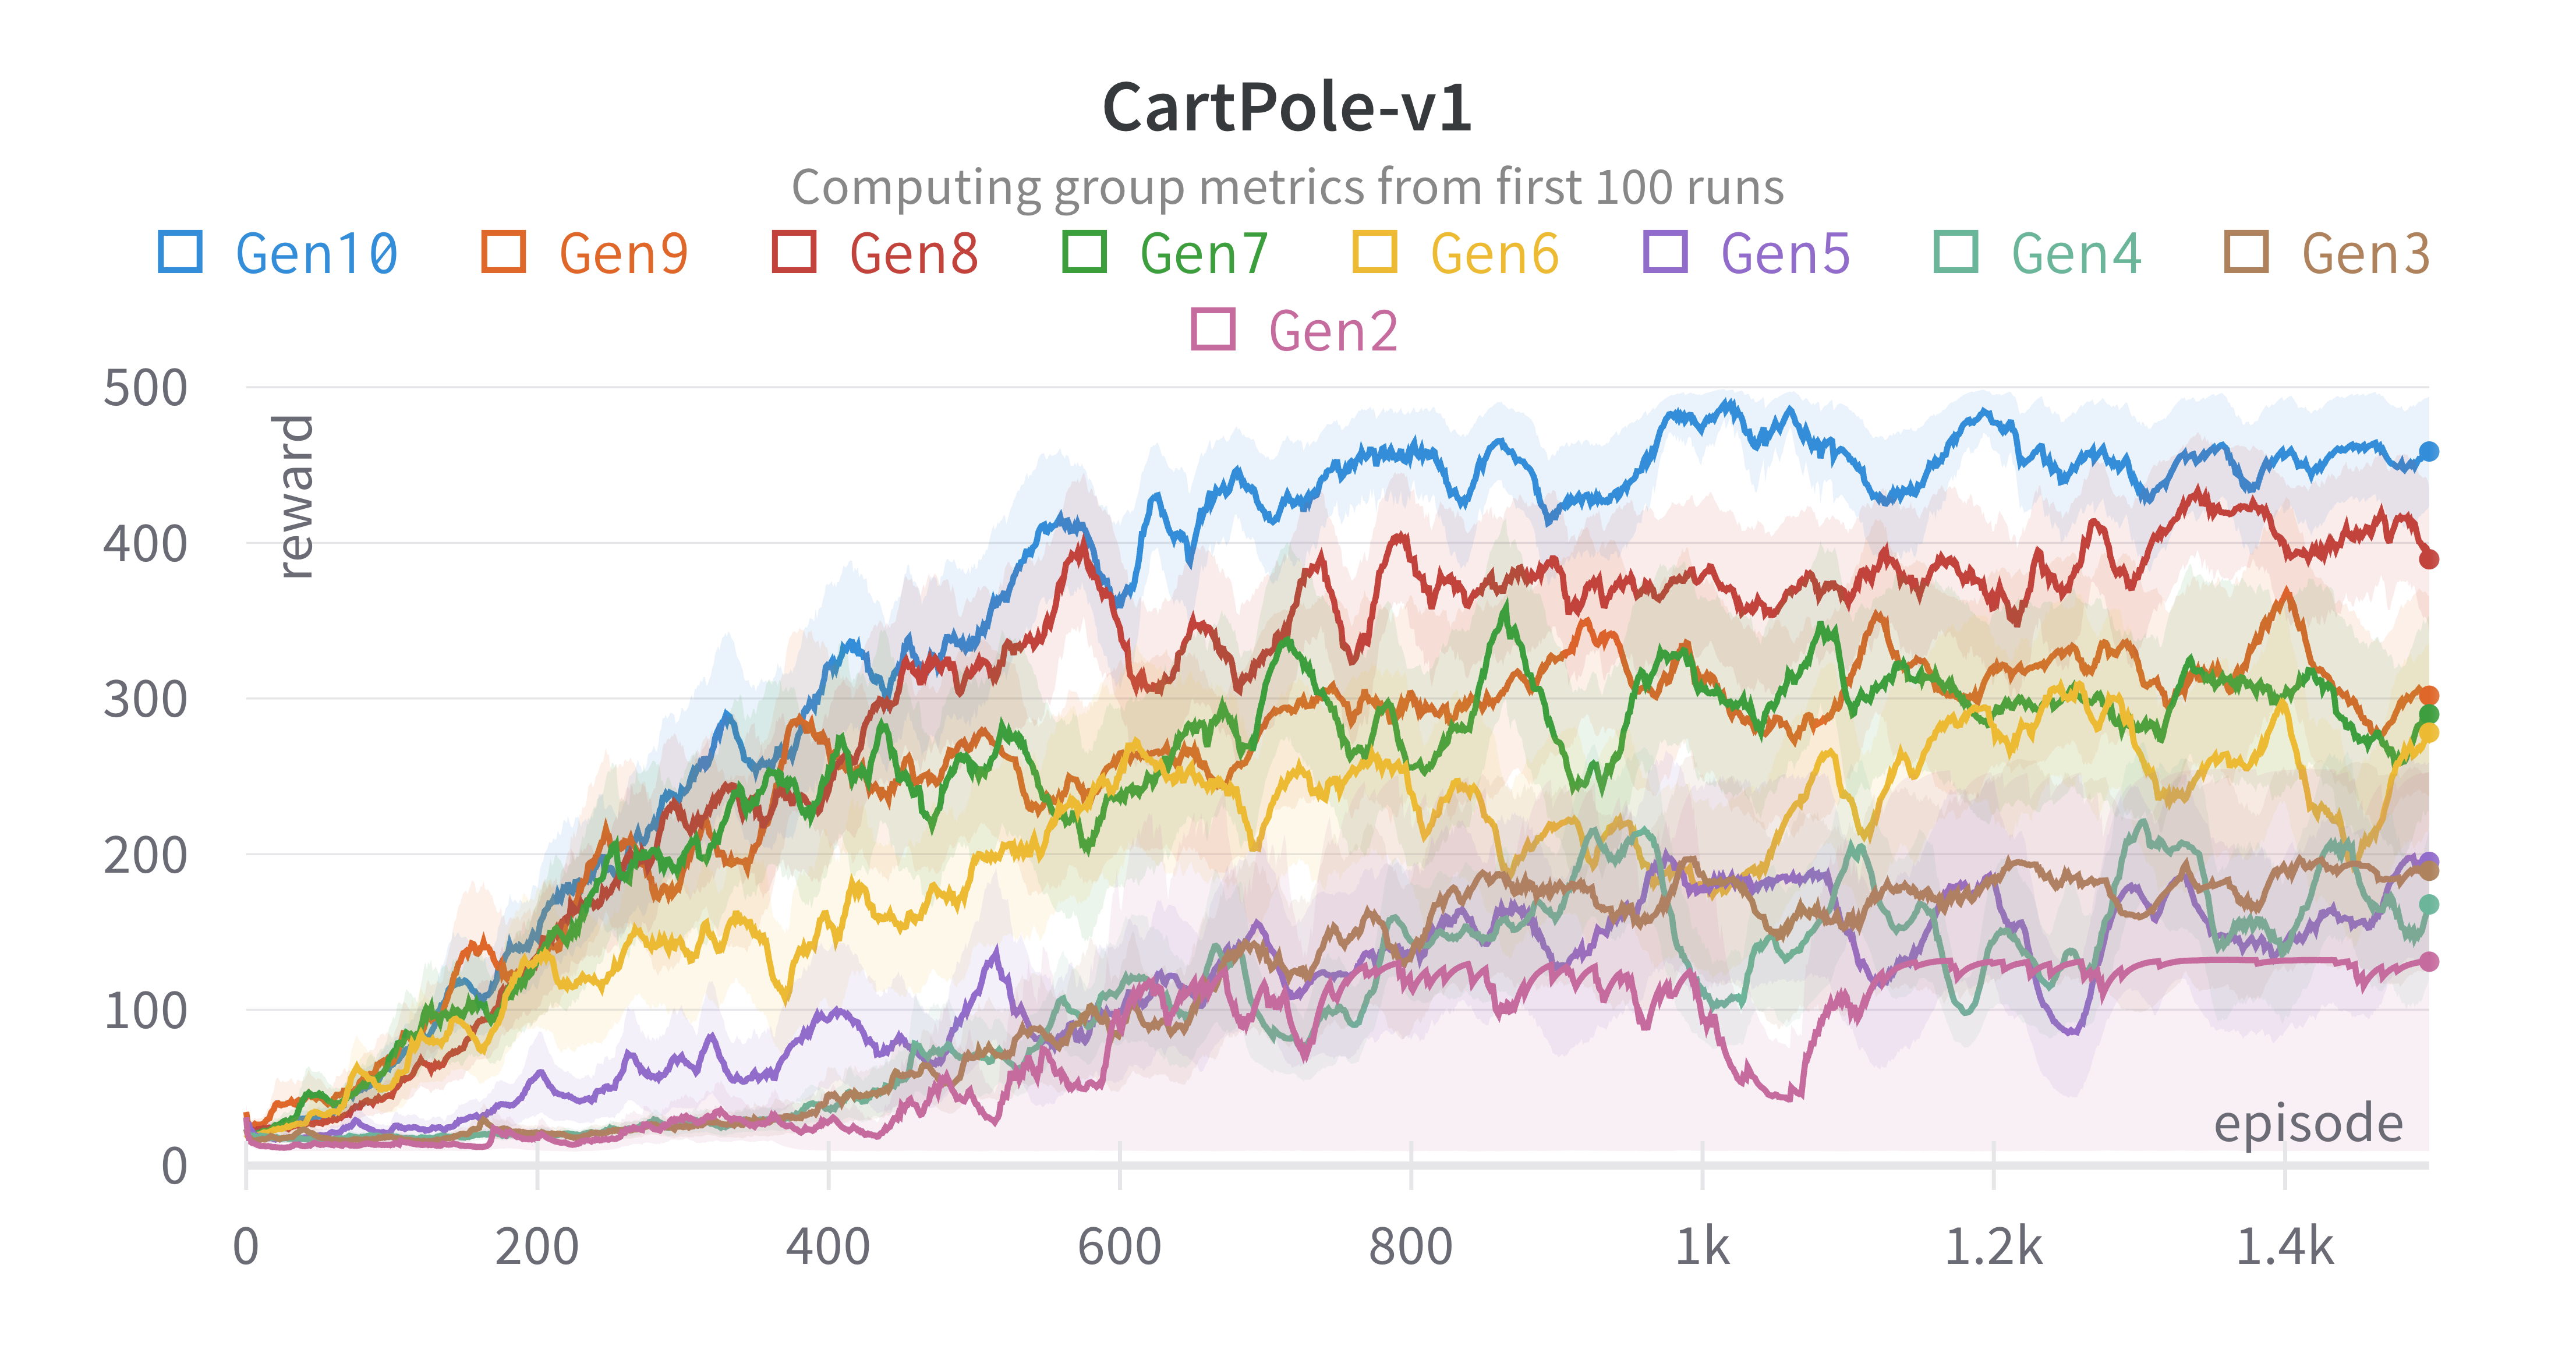
\includegraphics[width=0.9\linewidth]{figs/lc-cp.png}
    \caption{
        Be descriptive of what different colors/lines mean.
        A multi-line caption should be formatted as such.
        Try to not exceed 3 lines.
    }
    \label{fig:lc-cp}
\end{figure}

% -------------------------------------------------------------------
\subsection{Acrobot}
\label{ssec:ab}

\TODO{Lorem ipsum.}

% -------------------------------------------------------------------
\subsection{LunarLander}
\label{ssec:ll}

\TODO{Lorem ipsum.}

% -------------------------------------------------------------------
% -------------------------------------------------------------------
\section{Conclusion}
\label{sec:conc}

\TODO{
    What did we find, why are some architectures/params better than others for specific environment?
    Is EA a valid approach for this problem?
}

\section{Discussion}
\label{sec:disc}

\TODO{
    What could be improved?
    What could be done differently?
    What could be done next?
}

% -------------------------------------------------------------------
\bibliography{references}

\end{document}
